\documentclass[onecolumn,12pt]{article}
\usepackage[utf8]{inputenc}
\usepackage{amsmath,amssymb,MnSymbol,amsbsy,mathrsfs}
\usepackage{graphicx}
\bibliographystyle{plain}
\author{Oussama ENNAFII & Shuyu DONG}
\title{Dreem project: supervised learning on EEG signals for sleep stage detection}

\begin{document}
\maketitle
	
\section{Introduction}

	In this report, we describe an automatic method to detect the K-complex transient before it occurs. In practice, we have a $3s$-duration of an EEG recording and the objective is to predict whether or not, in the next $0.5s$, the K-complex transient would occur. Basicaly, we have to characterize the signals so as to classify them. We are in a supervised setting where the labels are given: i.e. we know what are the signals that preceed a K-transient. The application of this classification is of interest for the start-up Dreem as they need to detect beforehand the K-complex so as to stimulate the brain in time while this transient occurs. The goal is to make sleep more efficient. The signals we have are sampled at $200 Hz$ which means that we have $600$ samples. There are $4861$ samples that are positive (i.e. a K-complex occurs in the $0.5s$ after) out of $ 69550$, which makes up to $6.99\%$ in terms of percentage.\\
	
	\begin{figure}
		\centering
		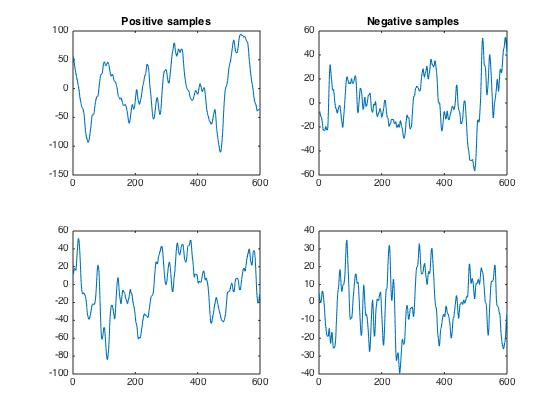
\includegraphics[scale=0.5]{samples}
		\caption{\label{fig:samples} Examples of positive and negative samples.}
	\end{figure}
	
	These samples do not need preprocessing. In fact, when using the Soft thresholding in the Daubechies wavelet basis we get a denoised signal that is too close to the original.(c.f figure ~\ref{fig:denoising}). So as to reduce the computation time we do not preprocess those signals.\\
	
	\begin{figure}
		\centering
		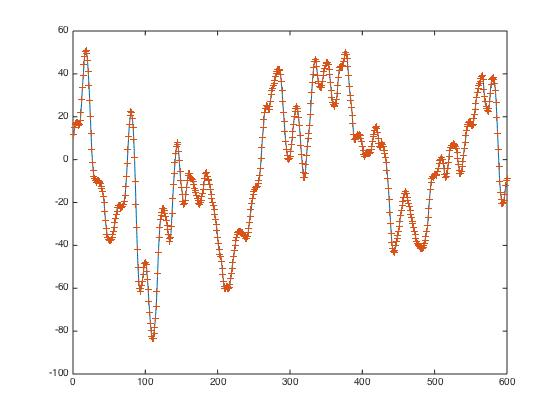
\includegraphics[scale=0.3]{denoise}
		\caption{\label{fig:denoising} In blue the original signal and in red the denoised one.}
	\end{figure}
	
	\section{Scattering}
	
	In order to classify the signals, we need a reliable way to represent it. So the idea is to construct a representation mapping $\Phi: \mathscr{C}^1([0,1]) \rightarrow \mathscr{H}$ to a feature space where the classification may be possible. In other words, we need a metric to compare signals $K(x,y)=<\Phi(x),\Phi(y)>$. This representation ought to be stable to small deformations: Let $\tau:[0,1] \rightarrow [0,1]$ a time deformation. We suppose that $\tau \in  \mathscr{C}^1([0,1]) $ and we define the time-wrapping for a signal $x$ : $x_{\tau}=x(\bullet- \tau(\bullet) )$
	
	\begin{equation}
	\begin{split}
		\exists C>0 \quad \forall x \in \mathscr{C}^1([0,1]) \quad  \forall \tau \in \mathscr{C}^1([0,1])  \quad \text{s.t. \ } ||\tau'||_{\infty}<1 \\
				 ||\Phi(x)-\Phi(x_{\tau})||\leq C ||\tau'||_{\infty} || x||
	\end{split}
	\end{equation}
	
	This Lipschitz property means that for small deformation ($||\tau'||_{\infty}<1 $)we can linearize the distance in the feature space of the two signals.\\
	
	For example, if we take the spectrogram:
	
	\begin{equation}
		|\hat{x}(t,\omega)|=|\int x(u) \phi(u-t) e^{-i\omega t} du|
	\end{equation}
	
	and a deformation: $\tau=\epsilon . \bullet $ where $\epsilon<1$. $$\hat{x_{\tau}}(\omega)=\frac{\hat{x}(\frac{\omega}{1-\epsilon})}{1-\epsilon}$$
	
	So of high frequencies in the signal are not negligeable, we can always find a frequency $\xi$ such that $\epsilon \xi$ is big enough to separate the two supports (c.f. figure ~\ref{fig:speccomp}). In this case the Lipschitz property do not hold. 
	
	\begin{figure}
		\centering
		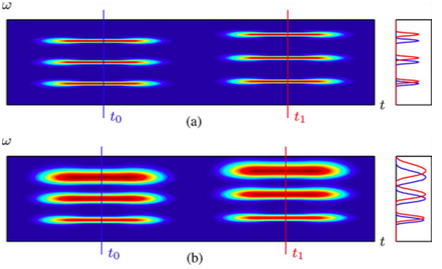
\includegraphics[scale=0.5]{speccomp}
		\caption{\label{fig:speccomp} Comparison between a spectorgram and a mel-frequency spectrum.}
	\end{figure}
	
	An idea so that we get stable representations is to cut-off high frequencies or more precisely to be interested in intervals of frequencies once at a time. This means that we need constant-$Q$ bandpass filters $\Psi_{\lambda}$ centered at $\lambda$ with a bandwidth of the order of $\frac{\lambda}{Q}$. At lower frequencies the bandwidth is constant: $\frac{2\pi }{T}$.Now the error is of order $\epsilon . Q$:
	
	\begin{equation}
		Mx(t,\lambda)=\int \hat{x}(t,\omega)|^2 \quad|\psi_{\lambda}(\omega)|^2 d\omega
	\end{equation}
	
	$T$, the window duration, is chosen small so as to be able to reconstruct the signal but in the same time we need a big window in order to understand the structure of the whole signal. In last setting, we lose too much information that we cannot reconstruct the signal. That is where the scattering transform intervenes. In fact, we are going to repeat the same thing for filtered signals before averaging.
	
	For this purpose, we are going to work with analytic wavelets $\psi$:
	$$\psi_{\lambda}=\lambda \psi(\lambda \bullet) \quad \text{and} \quad \widehat{\psi}_{\lambda}= \widehat{\psi}(\frac{\bullet}{\lambda})$$ 
	with $\lambda =2^{\frac{k}{Q}},\quad \forall k \in \mathbb{Z}$. The support of $\widehat{\Psi}_{\lambda}$ is centered at $\lambda$ with a bandwidth $\frac{\lambda}{Q}$. For low frequencies : $\lambda <\frac{2 \pi Q}{T}$ the bandwidth is constant: $\frac{2\pi}{T}$. 
	We introduce then the wavelet transform operator:
	\begin{equation}
		W x=(x\star \phi(t), x \star \psi_{\lambda}(t))_{\lambda \in \Lambda,t \in \mathbb{R}}
	\end{equation}
	
	We define:\\
	
	\begin{equation}
		A(\omega)=|\widehat{\phi}|^2+ \frac{1}{2} \sum_{\lambda \in \Lambda} (|\psi_{\lambda}(\omega)|^2 +|\psi_{\lambda}(-\omega)|^2)
	\end{equation}
	
	
		We choose $\psi$ and $\phi$ so that $A(\omega)=1$ which means that $||Wx||=1$ (by Plancherel's equality).$W$ is called tight frame operators. We define :
		$$\widehat{\bar{\phi}}=\frac{\widehat{\phi}^*}{A}\quad \text{and} \quad \widehat{\bar{\psi}}_{\lambda}=\frac{\widehat{\psi}_{\lambda}^*}{A}$$
		Now we can invert $W$ by (using Parseval equality):
		$$x(t)=x\star \phi \star \bar{\phi}(t) + \sum_{\lambda \in \Lambda} \mathscr{R}(x\star \psi_{\lambda} \star \bar{\psi}_{\lambda})$$
		
		Like in the demodulation, where we aim at separating the carrying frequency from the signal we use the modulus:
		
		$$|W| x= (x\star \phi(t), |x \star \psi_{\lambda}(t)|)_{\lambda \in \Lambda,t \in \mathbb{R}}$$
		
		This is a contraction since: $||\quad|W|x - |W|y\quad|| \leq ||x-y||$ 
		
		Now we have constructed an operator resembling the mel-frequency operator. To recover the information lost by the demodulation and averaging, the idea is to apply the modulus of the wavelet transform operator for $|x \star \psi_{\lambda}|$.\\
		
		We proceed by isolating: $S_0x(t)= x \star \phi(t)$ from the operator:
		
		$$|W_1| x= (x\star \phi(t), |x \star \psi_{\lambda_1}(t)|)_{\lambda _1\in \Lambda_1,t \in \mathbb{R}}$$
		
		We isolate then: $S_1x(t,\lambda_1)= |x \star \psi_{\lambda_1}|\star \phi(t)$ from the operator:
		
		$$|W_2| \text{\ . }|x \star \psi_{\lambda_1}|= (|x \star \psi_{\lambda_1}|\star \phi(t), ||x \star \psi_{\lambda_1}| \star \psi_{\lambda_2}(t)|)_{\lambda _2\in \Lambda_2,t \in \mathbb{R}}$$
		
		We continue doing the same thing for:
		\begin{eqnarray}
			U_m x(t,\lambda_1,\lambda_2,\dots,\lambda_m) &=& ||\dots|x \star \psi_{\lambda_1}|\star \psi_{\lambda_2}|\star \dots|\star \psi_{\lambda_m}|\\
			S_mx(t,\lambda_1,\lambda_2,\dots,\lambda_m)&=& U_mx(t,\lambda_1,\lambda_2,\dots,\lambda_m)\star \phi(t)\\
			|W_m| \text{\ . }U_mx&=& (S_mx,U_{m+1}x)
		\end{eqnarray}
		
		
		The scattering transform up to a level $l$ is then defined by:
		\begin{equation}
			S\text{\ . }x=(S_mx)_{m=1,\dots,l}
		\end{equation}
		
		and we illustrate it by a tree like in the figure ~\ref{fig:scat}.\\
		\begin{figure}
			\centering
			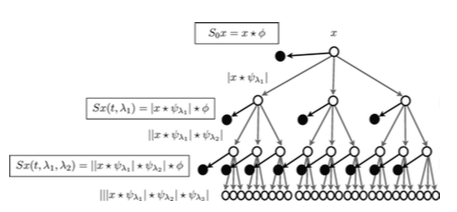
\includegraphics[scale=0.5]{scat}
			\caption{\label{fig:scat} Scattering transform.}
		\end{figure}
		
		The scattering transform is stable by time-wrap deformation:
		$$||S(x)-S(x_{\tau})||\leq C ||\tau'||_{\infty} || x||$$
		
		For morlet wavelets $C=2$.
		
		Since all $|W_m|$ are contractions we can prove that $S$ is a contraction too:
		
		$$||Sx-Sy|| \leq ||x-y||$$
	 Further, since $|W_m|$ preserves the norms:
	 
	 $$||x||^2=||Sx||^2+ ||U_{l+1}x||^2$$
	   We can prove that: $||U_{l+1}x|| \rightarrow 0$ when $l\rightarrow\infty$ i.e.
	   
	   $$||Sx||\rightarrow ||x||$$
	   
	   $S$ is also proven to be invertible when $l\rightarrow\infty$. This means that we can reconstruct the signal from $Sx$. In practice, we do not need too much levels, as wa can infere $l$ by comparing $||Sx||$ to $||x||$. The computations can be done using the FFT convolution which means that we need $O(\text{N.log(N)})$ flops.\\
	   
	   Afterwards, we normalize $S$ so as to have a more invariant representation.
	   
	   \begin{eqnarray}
	   	\tilde{S}_1x(t,\lambda_1)&=&\frac{S_1x(t,\lambda_1)}{|x|\star \phi(t)}\\
	   	\tilde{S}_mx(t,\lambda_1,\dots,\lambda_m)&=&\frac{S_mx(t,\lambda_1,\dots,\lambda_m)}{S_{m-1}x(t,\lambda_1,\dots,\lambda_{m-1})}
	   \end{eqnarray}
	
	Indeed, $S_1$ becomes invariant to multiplicative constants, while $S_2$ becomes invariant to filtering by $\widehat{h}$ that is constant over its support. In the end, we appy the natural logarithm to consider the fractal dynamics aspect for the classification. That is because the scatterring coefficients have a power-law behaviors:
	$$S_1x(j_1,k)=2^{ jz_1(k)}$$
	$$\tilde{S}_2x(j_1,j_2,k)=2^{(j_2-j_1)z_2(j_1,k)}$$
	
	for scale invariant processes $z_2$ is shown to be independent from $j_2$.In general, the larger the $z_2 (j_1 )$, the more bursty in time the data. The $z_2 (j_1 )$ is then called the intermittency scaling exponents. In the other hand, $z_1$ gives a global regularity information which mostly depends upon its second-order statistics.
	
	\section{References:}
	~\\
	\begin{itemize}
		\item[[1]] Scattering Transform for Intrapartum Fetal Heart Rate, Variability Fractal Analysis: A Case-
		Control Study Vaclav Chudacek, Joakim Anden, Stéphane Mallat, Fellow, IEEE, Patrice Abry, Fellow, IEEE, and Muriel DoretIEEE TRANSACTIONS ON BIOMEDICAL ENGINEERING, VOL. 61, NO. 4, APRIL 2014\\
		
		\item[[2]] Deep Scattering Spectrum, Joakin Anden Member, IEEE, and Stéphane Mallat Fellow, IEEE, IEEE Transactions on signal processing, VOL.62, NO.16, AUGUST 15, 2014\\
		
		\item[[3]] Wavelet EEG Denoising for automatic sleep stage classification, Edson Estrada, Homer Nazeran, Gustavo Sierra, Farideh Ebrahimi, Mohammed Mikaeili, University of Texas El Paso, Department of Electrical and Computer Engineering, El Pasto TX, USA, Universidad Autonoma de Ciudad Juarez, Instituto de Ciencias Biomédicas, Cd. Juarez, Chih, Mexico 3Shahed University, Depart-
		ment of Biomedical Engineering, Tehran I R IRAN
	\end{itemize}
	
\end{document}